% Created by tikzDevice version 0.12.6 on 2025-04-15 12:19:28
% !TEX encoding = UTF-8 Unicode
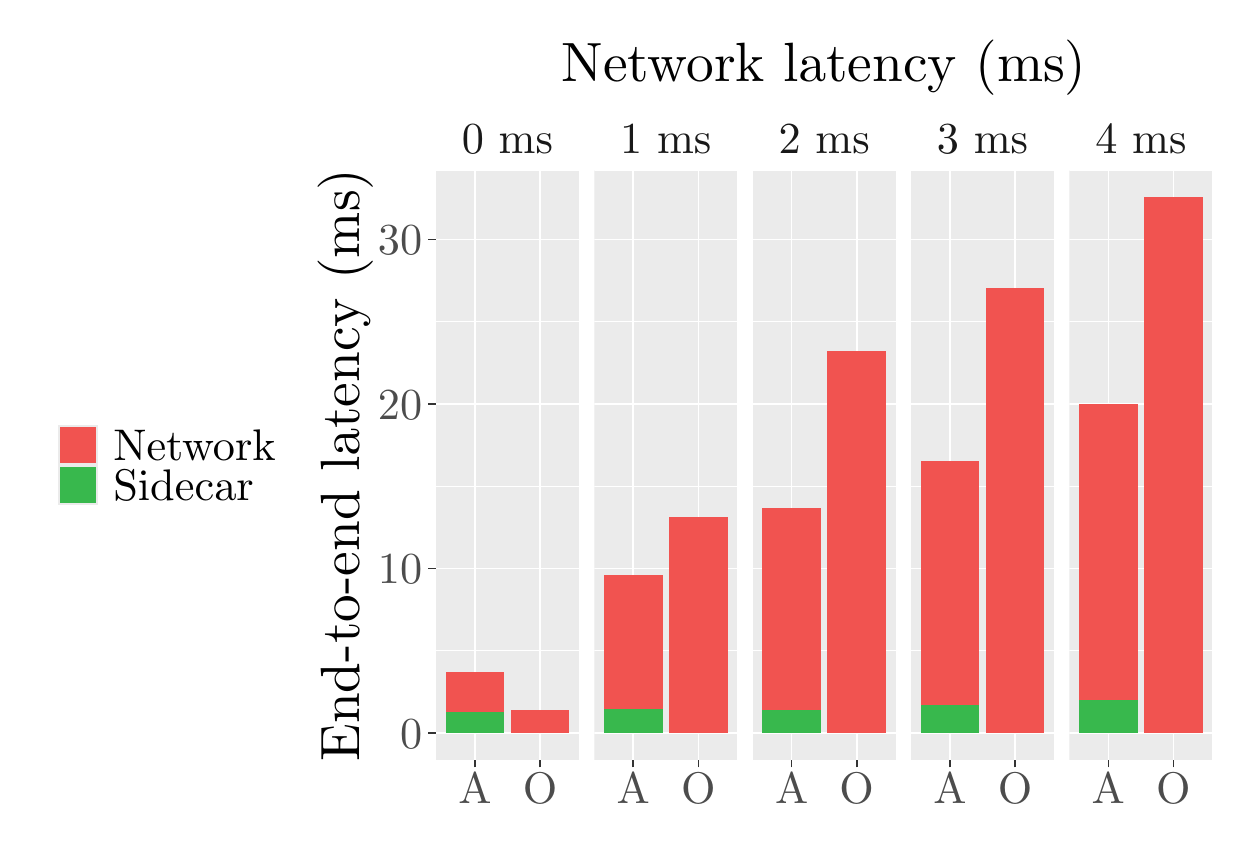
\begin{tikzpicture}[x=1pt,y=1pt]
\definecolor{fillColor}{RGB}{255,255,255}
\path[use as bounding box,fill=fillColor,fill opacity=0.00] (0,0) rectangle (433.62,289.08);
\begin{scope}
\path[clip] (  0.00,  0.00) rectangle (433.62,289.08);
\definecolor{drawColor}{RGB}{255,255,255}
\definecolor{fillColor}{RGB}{255,255,255}

\path[draw=drawColor,line width= 0.6pt,line join=round,line cap=round,fill=fillColor] (  0.00,  0.00) rectangle (433.62,289.08);
\end{scope}
\begin{scope}
\path[clip] (147.51, 24.58) rectangle (199.23,237.49);
\definecolor{fillColor}{gray}{0.92}

\path[fill=fillColor] (147.51, 24.58) rectangle (199.23,237.49);
\definecolor{drawColor}{RGB}{255,255,255}

\path[draw=drawColor,line width= 0.3pt,line join=round] (147.51, 63.96) --
	(199.23, 63.96);

\path[draw=drawColor,line width= 0.3pt,line join=round] (147.51,123.37) --
	(199.23,123.37);

\path[draw=drawColor,line width= 0.3pt,line join=round] (147.51,182.78) --
	(199.23,182.78);

\path[draw=drawColor,line width= 0.6pt,line join=round] (147.51, 34.26) --
	(199.23, 34.26);

\path[draw=drawColor,line width= 0.6pt,line join=round] (147.51, 93.67) --
	(199.23, 93.67);

\path[draw=drawColor,line width= 0.6pt,line join=round] (147.51,153.08) --
	(199.23,153.08);

\path[draw=drawColor,line width= 0.6pt,line join=round] (147.51,212.49) --
	(199.23,212.49);

\path[draw=drawColor,line width= 0.6pt,line join=round] (161.62, 24.58) --
	(161.62,237.49);

\path[draw=drawColor,line width= 0.6pt,line join=round] (185.13, 24.58) --
	(185.13,237.49);
\definecolor{fillColor}{RGB}{241,83,80}

\path[fill=fillColor] (174.55, 34.26) rectangle (195.71, 42.44);
\definecolor{fillColor}{RGB}{56,184,77}

\path[fill=fillColor] (151.04, 34.26) rectangle (172.20, 41.97);
\definecolor{fillColor}{RGB}{241,83,80}

\path[fill=fillColor] (151.04, 41.97) rectangle (172.20, 56.41);
\end{scope}
\begin{scope}
\path[clip] (204.73, 24.58) rectangle (256.45,237.49);
\definecolor{fillColor}{gray}{0.92}

\path[fill=fillColor] (204.73, 24.58) rectangle (256.45,237.49);
\definecolor{drawColor}{RGB}{255,255,255}

\path[draw=drawColor,line width= 0.3pt,line join=round] (204.73, 63.96) --
	(256.45, 63.96);

\path[draw=drawColor,line width= 0.3pt,line join=round] (204.73,123.37) --
	(256.45,123.37);

\path[draw=drawColor,line width= 0.3pt,line join=round] (204.73,182.78) --
	(256.45,182.78);

\path[draw=drawColor,line width= 0.6pt,line join=round] (204.73, 34.26) --
	(256.45, 34.26);

\path[draw=drawColor,line width= 0.6pt,line join=round] (204.73, 93.67) --
	(256.45, 93.67);

\path[draw=drawColor,line width= 0.6pt,line join=round] (204.73,153.08) --
	(256.45,153.08);

\path[draw=drawColor,line width= 0.6pt,line join=round] (204.73,212.49) --
	(256.45,212.49);

\path[draw=drawColor,line width= 0.6pt,line join=round] (218.84, 24.58) --
	(218.84,237.49);

\path[draw=drawColor,line width= 0.6pt,line join=round] (242.35, 24.58) --
	(242.35,237.49);
\definecolor{fillColor}{RGB}{241,83,80}

\path[fill=fillColor] (231.77, 34.26) rectangle (252.93,112.14);
\definecolor{fillColor}{RGB}{56,184,77}

\path[fill=fillColor] (208.26, 34.26) rectangle (229.42, 42.95);
\definecolor{fillColor}{RGB}{241,83,80}

\path[fill=fillColor] (208.26, 42.95) rectangle (229.42, 91.43);
\end{scope}
\begin{scope}
\path[clip] (261.95, 24.58) rectangle (313.68,237.49);
\definecolor{fillColor}{gray}{0.92}

\path[fill=fillColor] (261.95, 24.58) rectangle (313.68,237.49);
\definecolor{drawColor}{RGB}{255,255,255}

\path[draw=drawColor,line width= 0.3pt,line join=round] (261.95, 63.96) --
	(313.68, 63.96);

\path[draw=drawColor,line width= 0.3pt,line join=round] (261.95,123.37) --
	(313.68,123.37);

\path[draw=drawColor,line width= 0.3pt,line join=round] (261.95,182.78) --
	(313.68,182.78);

\path[draw=drawColor,line width= 0.6pt,line join=round] (261.95, 34.26) --
	(313.68, 34.26);

\path[draw=drawColor,line width= 0.6pt,line join=round] (261.95, 93.67) --
	(313.68, 93.67);

\path[draw=drawColor,line width= 0.6pt,line join=round] (261.95,153.08) --
	(313.68,153.08);

\path[draw=drawColor,line width= 0.6pt,line join=round] (261.95,212.49) --
	(313.68,212.49);

\path[draw=drawColor,line width= 0.6pt,line join=round] (276.06, 24.58) --
	(276.06,237.49);

\path[draw=drawColor,line width= 0.6pt,line join=round] (299.57, 24.58) --
	(299.57,237.49);
\definecolor{fillColor}{RGB}{241,83,80}

\path[fill=fillColor] (288.99, 34.26) rectangle (310.15,172.18);
\definecolor{fillColor}{RGB}{56,184,77}

\path[fill=fillColor] (265.48, 34.26) rectangle (286.64, 42.38);
\definecolor{fillColor}{RGB}{241,83,80}

\path[fill=fillColor] (265.48, 42.38) rectangle (286.64,115.69);
\end{scope}
\begin{scope}
\path[clip] (319.18, 24.58) rectangle (370.90,237.49);
\definecolor{fillColor}{gray}{0.92}

\path[fill=fillColor] (319.18, 24.58) rectangle (370.90,237.49);
\definecolor{drawColor}{RGB}{255,255,255}

\path[draw=drawColor,line width= 0.3pt,line join=round] (319.18, 63.96) --
	(370.90, 63.96);

\path[draw=drawColor,line width= 0.3pt,line join=round] (319.18,123.37) --
	(370.90,123.37);

\path[draw=drawColor,line width= 0.3pt,line join=round] (319.18,182.78) --
	(370.90,182.78);

\path[draw=drawColor,line width= 0.6pt,line join=round] (319.18, 34.26) --
	(370.90, 34.26);

\path[draw=drawColor,line width= 0.6pt,line join=round] (319.18, 93.67) --
	(370.90, 93.67);

\path[draw=drawColor,line width= 0.6pt,line join=round] (319.18,153.08) --
	(370.90,153.08);

\path[draw=drawColor,line width= 0.6pt,line join=round] (319.18,212.49) --
	(370.90,212.49);

\path[draw=drawColor,line width= 0.6pt,line join=round] (333.28, 24.58) --
	(333.28,237.49);

\path[draw=drawColor,line width= 0.6pt,line join=round] (356.79, 24.58) --
	(356.79,237.49);
\definecolor{fillColor}{RGB}{241,83,80}

\path[fill=fillColor] (346.21, 34.26) rectangle (367.37,195.02);
\definecolor{fillColor}{RGB}{56,184,77}

\path[fill=fillColor] (322.70, 34.26) rectangle (343.86, 44.23);
\definecolor{fillColor}{RGB}{241,83,80}

\path[fill=fillColor] (322.70, 44.23) rectangle (343.86,132.63);
\end{scope}
\begin{scope}
\path[clip] (376.40, 24.58) rectangle (428.12,237.49);
\definecolor{fillColor}{gray}{0.92}

\path[fill=fillColor] (376.40, 24.58) rectangle (428.12,237.49);
\definecolor{drawColor}{RGB}{255,255,255}

\path[draw=drawColor,line width= 0.3pt,line join=round] (376.40, 63.96) --
	(428.12, 63.96);

\path[draw=drawColor,line width= 0.3pt,line join=round] (376.40,123.37) --
	(428.12,123.37);

\path[draw=drawColor,line width= 0.3pt,line join=round] (376.40,182.78) --
	(428.12,182.78);

\path[draw=drawColor,line width= 0.6pt,line join=round] (376.40, 34.26) --
	(428.12, 34.26);

\path[draw=drawColor,line width= 0.6pt,line join=round] (376.40, 93.67) --
	(428.12, 93.67);

\path[draw=drawColor,line width= 0.6pt,line join=round] (376.40,153.08) --
	(428.12,153.08);

\path[draw=drawColor,line width= 0.6pt,line join=round] (376.40,212.49) --
	(428.12,212.49);

\path[draw=drawColor,line width= 0.6pt,line join=round] (390.50, 24.58) --
	(390.50,237.49);

\path[draw=drawColor,line width= 0.6pt,line join=round] (414.01, 24.58) --
	(414.01,237.49);
\definecolor{fillColor}{RGB}{241,83,80}

\path[fill=fillColor] (403.43, 34.26) rectangle (424.59,227.81);
\definecolor{fillColor}{RGB}{56,184,77}

\path[fill=fillColor] (379.92, 34.26) rectangle (401.08, 46.11);
\definecolor{fillColor}{RGB}{241,83,80}

\path[fill=fillColor] (379.92, 46.11) rectangle (401.08,153.02);
\end{scope}
\begin{scope}
\path[clip] (147.51,237.49) rectangle (199.23,260.42);
\definecolor{drawColor}{RGB}{255,255,255}

\path[draw=drawColor,line width= 0.6pt,line join=round,line cap=round] (147.51,237.49) rectangle (199.23,260.42);
\definecolor{drawColor}{gray}{0.10}

\node[text=drawColor,anchor=base,inner sep=0pt, outer sep=0pt, scale=  1.60] at (173.37,243.44) {0 ms};
\end{scope}
\begin{scope}
\path[clip] (204.73,237.49) rectangle (256.45,260.42);
\definecolor{drawColor}{RGB}{255,255,255}

\path[draw=drawColor,line width= 0.6pt,line join=round,line cap=round] (204.73,237.49) rectangle (256.45,260.42);
\definecolor{drawColor}{gray}{0.10}

\node[text=drawColor,anchor=base,inner sep=0pt, outer sep=0pt, scale=  1.60] at (230.59,243.44) {1 ms};
\end{scope}
\begin{scope}
\path[clip] (261.95,237.49) rectangle (313.68,260.42);
\definecolor{drawColor}{RGB}{255,255,255}

\path[draw=drawColor,line width= 0.6pt,line join=round,line cap=round] (261.95,237.49) rectangle (313.68,260.42);
\definecolor{drawColor}{gray}{0.10}

\node[text=drawColor,anchor=base,inner sep=0pt, outer sep=0pt, scale=  1.60] at (287.81,243.44) {2 ms};
\end{scope}
\begin{scope}
\path[clip] (319.18,237.49) rectangle (370.90,260.42);
\definecolor{drawColor}{RGB}{255,255,255}

\path[draw=drawColor,line width= 0.6pt,line join=round,line cap=round] (319.18,237.49) rectangle (370.90,260.42);
\definecolor{drawColor}{gray}{0.10}

\node[text=drawColor,anchor=base,inner sep=0pt, outer sep=0pt, scale=  1.60] at (345.04,243.44) {3 ms};
\end{scope}
\begin{scope}
\path[clip] (376.40,237.49) rectangle (428.12,260.42);
\definecolor{drawColor}{RGB}{255,255,255}

\path[draw=drawColor,line width= 0.6pt,line join=round,line cap=round] (376.40,237.49) rectangle (428.12,260.42);
\definecolor{drawColor}{gray}{0.10}

\node[text=drawColor,anchor=base,inner sep=0pt, outer sep=0pt, scale=  1.60] at (402.26,243.44) {4 ms};
\end{scope}
\begin{scope}
\path[clip] (  0.00,  0.00) rectangle (433.62,289.08);
\definecolor{drawColor}{gray}{0.20}

\path[draw=drawColor,line width= 0.6pt,line join=round] (161.62, 21.83) --
	(161.62, 24.58);

\path[draw=drawColor,line width= 0.6pt,line join=round] (185.13, 21.83) --
	(185.13, 24.58);
\end{scope}
\begin{scope}
\path[clip] (  0.00,  0.00) rectangle (433.62,289.08);
\definecolor{drawColor}{gray}{0.30}

\node[text=drawColor,anchor=base,inner sep=0pt, outer sep=0pt, scale=  1.60] at (161.62,  8.61) {A};

\node[text=drawColor,anchor=base,inner sep=0pt, outer sep=0pt, scale=  1.60] at (185.13,  8.61) {O};
\end{scope}
\begin{scope}
\path[clip] (  0.00,  0.00) rectangle (433.62,289.08);
\definecolor{drawColor}{gray}{0.20}

\path[draw=drawColor,line width= 0.6pt,line join=round] (218.84, 21.83) --
	(218.84, 24.58);

\path[draw=drawColor,line width= 0.6pt,line join=round] (242.35, 21.83) --
	(242.35, 24.58);
\end{scope}
\begin{scope}
\path[clip] (  0.00,  0.00) rectangle (433.62,289.08);
\definecolor{drawColor}{gray}{0.30}

\node[text=drawColor,anchor=base,inner sep=0pt, outer sep=0pt, scale=  1.60] at (218.84,  8.61) {A};

\node[text=drawColor,anchor=base,inner sep=0pt, outer sep=0pt, scale=  1.60] at (242.35,  8.61) {O};
\end{scope}
\begin{scope}
\path[clip] (  0.00,  0.00) rectangle (433.62,289.08);
\definecolor{drawColor}{gray}{0.20}

\path[draw=drawColor,line width= 0.6pt,line join=round] (276.06, 21.83) --
	(276.06, 24.58);

\path[draw=drawColor,line width= 0.6pt,line join=round] (299.57, 21.83) --
	(299.57, 24.58);
\end{scope}
\begin{scope}
\path[clip] (  0.00,  0.00) rectangle (433.62,289.08);
\definecolor{drawColor}{gray}{0.30}

\node[text=drawColor,anchor=base,inner sep=0pt, outer sep=0pt, scale=  1.60] at (276.06,  8.61) {A};

\node[text=drawColor,anchor=base,inner sep=0pt, outer sep=0pt, scale=  1.60] at (299.57,  8.61) {O};
\end{scope}
\begin{scope}
\path[clip] (  0.00,  0.00) rectangle (433.62,289.08);
\definecolor{drawColor}{gray}{0.20}

\path[draw=drawColor,line width= 0.6pt,line join=round] (333.28, 21.83) --
	(333.28, 24.58);

\path[draw=drawColor,line width= 0.6pt,line join=round] (356.79, 21.83) --
	(356.79, 24.58);
\end{scope}
\begin{scope}
\path[clip] (  0.00,  0.00) rectangle (433.62,289.08);
\definecolor{drawColor}{gray}{0.30}

\node[text=drawColor,anchor=base,inner sep=0pt, outer sep=0pt, scale=  1.60] at (333.28,  8.61) {A};

\node[text=drawColor,anchor=base,inner sep=0pt, outer sep=0pt, scale=  1.60] at (356.79,  8.61) {O};
\end{scope}
\begin{scope}
\path[clip] (  0.00,  0.00) rectangle (433.62,289.08);
\definecolor{drawColor}{gray}{0.20}

\path[draw=drawColor,line width= 0.6pt,line join=round] (390.50, 21.83) --
	(390.50, 24.58);

\path[draw=drawColor,line width= 0.6pt,line join=round] (414.01, 21.83) --
	(414.01, 24.58);
\end{scope}
\begin{scope}
\path[clip] (  0.00,  0.00) rectangle (433.62,289.08);
\definecolor{drawColor}{gray}{0.30}

\node[text=drawColor,anchor=base,inner sep=0pt, outer sep=0pt, scale=  1.60] at (390.50,  8.61) {A};

\node[text=drawColor,anchor=base,inner sep=0pt, outer sep=0pt, scale=  1.60] at (414.01,  8.61) {O};
\end{scope}
\begin{scope}
\path[clip] (  0.00,  0.00) rectangle (433.62,289.08);
\definecolor{drawColor}{gray}{0.30}

\node[text=drawColor,anchor=base east,inner sep=0pt, outer sep=0pt, scale=  1.60] at (142.56, 28.75) {0};

\node[text=drawColor,anchor=base east,inner sep=0pt, outer sep=0pt, scale=  1.60] at (142.56, 88.16) {10};

\node[text=drawColor,anchor=base east,inner sep=0pt, outer sep=0pt, scale=  1.60] at (142.56,147.57) {20};

\node[text=drawColor,anchor=base east,inner sep=0pt, outer sep=0pt, scale=  1.60] at (142.56,206.98) {30};
\end{scope}
\begin{scope}
\path[clip] (  0.00,  0.00) rectangle (433.62,289.08);
\definecolor{drawColor}{gray}{0.20}

\path[draw=drawColor,line width= 0.6pt,line join=round] (144.76, 34.26) --
	(147.51, 34.26);

\path[draw=drawColor,line width= 0.6pt,line join=round] (144.76, 93.67) --
	(147.51, 93.67);

\path[draw=drawColor,line width= 0.6pt,line join=round] (144.76,153.08) --
	(147.51,153.08);

\path[draw=drawColor,line width= 0.6pt,line join=round] (144.76,212.49) --
	(147.51,212.49);
\end{scope}
\begin{scope}
\path[clip] (  0.00,  0.00) rectangle (433.62,289.08);
\definecolor{drawColor}{RGB}{0,0,0}

\node[text=drawColor,rotate= 90.00,anchor=base,inner sep=0pt, outer sep=0pt, scale=  2.00] at (119.93,131.03) {End-to-end latency (ms)};
\end{scope}
\begin{scope}
\path[clip] (  0.00,  0.00) rectangle (433.62,289.08);
\definecolor{fillColor}{RGB}{255,255,255}

\path[fill=fillColor] (  5.50,111.08) rectangle ( 95.15,150.99);
\end{scope}
\begin{scope}
\path[clip] (  0.00,  0.00) rectangle (433.62,289.08);
\definecolor{fillColor}{gray}{0.92}

\path[fill=fillColor] ( 11.00,131.03) rectangle ( 25.45,145.49);
\end{scope}
\begin{scope}
\path[clip] (  0.00,  0.00) rectangle (433.62,289.08);
\definecolor{fillColor}{RGB}{241,83,80}

\path[fill=fillColor] ( 11.71,131.75) rectangle ( 24.74,144.78);
\end{scope}
\begin{scope}
\path[clip] (  0.00,  0.00) rectangle (433.62,289.08);
\definecolor{fillColor}{gray}{0.92}

\path[fill=fillColor] ( 11.00,116.58) rectangle ( 25.45,131.03);
\end{scope}
\begin{scope}
\path[clip] (  0.00,  0.00) rectangle (433.62,289.08);
\definecolor{fillColor}{RGB}{56,184,77}

\path[fill=fillColor] ( 11.71,117.29) rectangle ( 24.74,130.32);
\end{scope}
\begin{scope}
\path[clip] (  0.00,  0.00) rectangle (433.62,289.08);
\definecolor{drawColor}{RGB}{0,0,0}

\node[text=drawColor,anchor=base west,inner sep=0pt, outer sep=0pt, scale=  1.60] at ( 30.95,132.75) {Network};
\end{scope}
\begin{scope}
\path[clip] (  0.00,  0.00) rectangle (433.62,289.08);
\definecolor{drawColor}{RGB}{0,0,0}

\node[text=drawColor,anchor=base west,inner sep=0pt, outer sep=0pt, scale=  1.60] at ( 30.95,118.30) {Sidecar};
\end{scope}
\begin{scope}
\path[clip] (  0.00,  0.00) rectangle (433.62,289.08);
\definecolor{drawColor}{RGB}{0,0,0}

\node[text=drawColor,anchor=base,inner sep=0pt, outer sep=0pt, scale=  2.00] at (287.81,269.81) {Network latency (ms)};
\end{scope}
\end{tikzpicture}
